\chapter{Annexe C: Parsing JSON tree structure to the JIT}
\paragraph*{}
The tree structure that feeds the spacetree, hypertree, treemap and rgraph visualizations[W15] is always the same. Roughly speaking, the JSON tree structure consists of tree nodes, each having as properties:
\begin{itemize}
\item id a unique identifier for the node.
\item name a node's name.
\item data The data property contains a dataset. That is, an array of key-value objects defined by the user.
\end{itemize}
\paragraph*{}
Roughly speaking, this is where you can put some extra information about your node. You'll be able to access this information at different stages of the computation of the JIT visualizations by using a controller.
children An array of children nodes, or an empty array if the node is a leaf node. For example:
\begin{center}
\begin{figure}
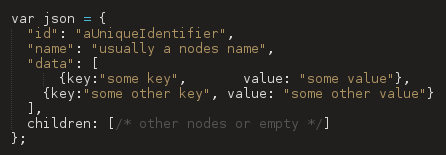
\includegraphics[scale=0.5]{example1.png}
\caption{Example of JSON strucutre}
\end{figure}
\end{center}
\paragraph*{}
\textbf{About datasets:} Sometimes some dataset objects are read by the JIT classes to perform proper layouts. For example, the treemap class reads the first object's value for each node's dataset to perform calculations about the dimensions of the rectangles laid. Also, if you enable the Config.Color.allow property, the treemap will add colors on the layout, and these colors will be based on your second dataset object value. \textbf{RGraphs} and Hyperbolic Trees also read the first dataset object value in order to compute node diameters and angular widths, when setting Config.allowVariableNodeDiameters = true. That's all for now. I recommend you to read the On controllers section and then some spacetree, hypertree, treemap or RGraph tutorials.
\paragraph*{}
\textbf{how to set the RGraph up and running:} the RGraph is inspired by Animated Exploration of Dynamic Graphs with Radial Layout (Ka-Ping Yee, Danyel Fisher, Rachna Dhamija, Marti Hearst) \url{http://bailando.sims.berkeley.edu/papers/infovis01.htm}
This visualization was built and engineered from scratch, taking only the paper as inspiration, and only shares some features with the visualization described in the paper.
Now for the implementation we are going to work with this tree JSON structure: 
\newpage
\begin{figure}[h]
\centering
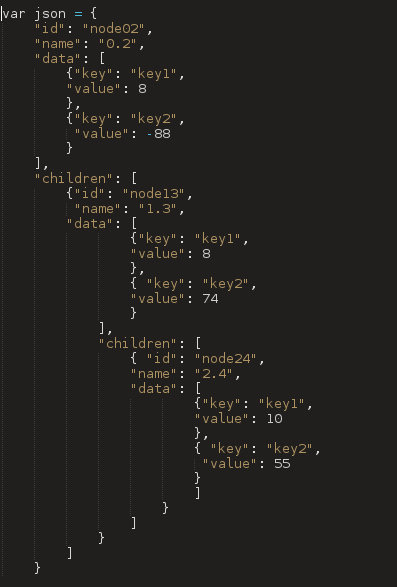
\includegraphics[scale=0.5]{example2.png}
\caption{tree JSON strcuture}
\end{figure}

\paragraph*{}
Put this HTML in your page: 

\begin{figure}[h]
\centering
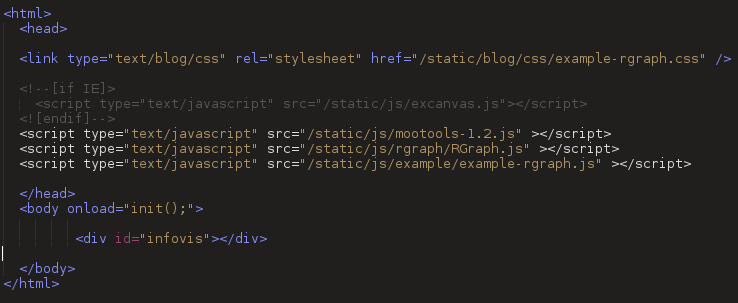
\includegraphics[scale=0.5]{htmlpage.png}
\caption{HTML page}
\end{figure}
\newpage
\paragraph*{}
You'll probably have to change the paths to the css and javascript files. Now, create a rgraph-example.css and put this code in it:

\begin{figure}[h]
\centering
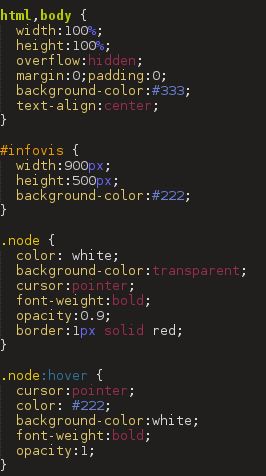
\includegraphics[scale=0.5]{csspage.png}
\caption{CSS RGraph}
\end{figure}

Finally, create an example-rgraph.js file and put this code in it:
\newpage
\begin{figure}[h]
\centering
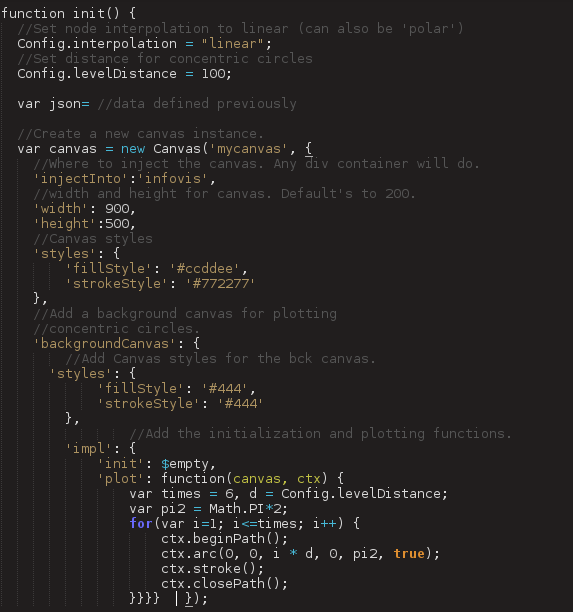
\includegraphics[scale=0.5]{rgraphjs1.png}
\end{figure}
\begin{figure}[h]
\centering
\includegraphics[scale=0.5]{rgraphjs2.png}
\end{figure}
\newpage
\paragraph*{}
You should see a RGraph up and running. Click on the labels and the tree should move. By assigning false to the backgroundCanvas property you can strip off the concentric circles. The backgroundCanvas functions and styles can also be customized to plot whatever background you like. Alsow e can add some JavaScript controller [W16] in order to put the name of the nodes into the labels. We need to use the onCreateLabel method
\begin{figure}[h]
\centering
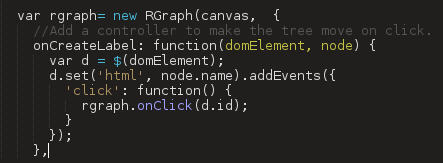
\includegraphics[scale=0.5]{controller.png}
\end{figure}
\paragraph*{}
For more information about the controller on RGraph tools you can visit this API docuementation [W17] created by Nicolas 